%
% $LastChangedRevision: 2085 $
% $LastChangedDate:: 2020-11-09 10:05:23 +0100#$
%
% This file is part of X2C. http://x2c.lcm.at/
%
% ===== CONFIDENTIAL =====
% The content of this file is confidential according to the X2C Licence Terms and Conditions.
%
% Copyright (c) 2020, Linz Center of Mechatronics GmbH (LCM) http://www.lcm.at/
% All rights reserved.
%
\textbf{Procedure}:\\
The algorithm is based on the paper \textit{"Initial rotor angle detection of a nonsalient pole permanent magnet synchronous machine"} by P.B. Schmidt, M. Gasperi, G. Ray, Gorby and A.H. Wijenayake from 1997.
\begin{figure}[H]
	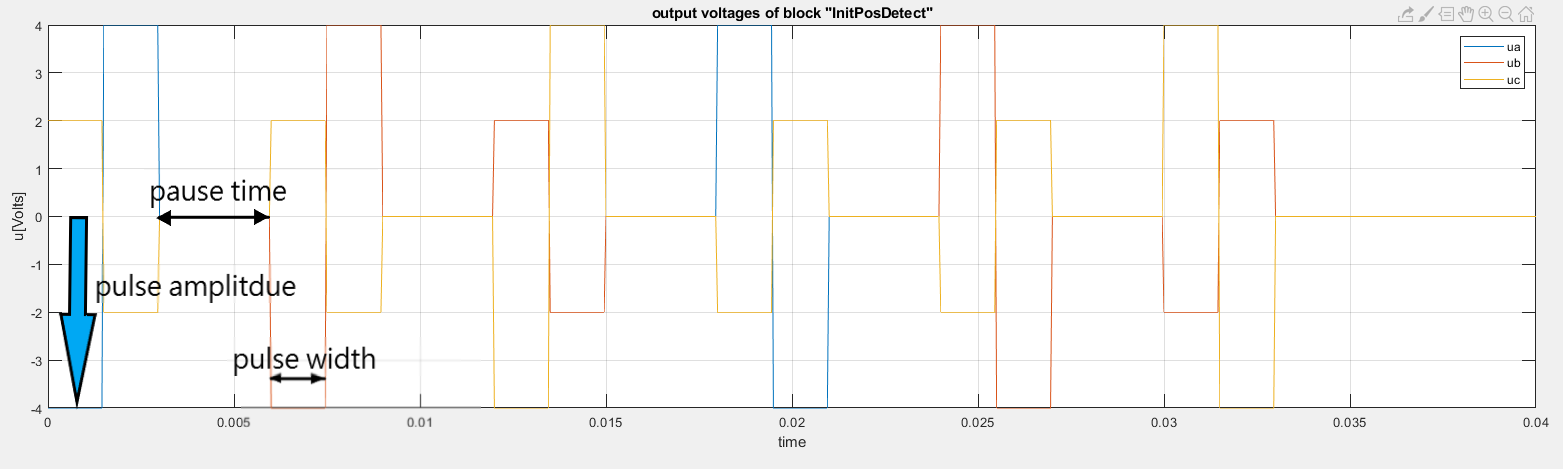
\includegraphics[width=\textwidth]{VoltagePulses}
	\caption{Voltage pulses over time. A counter pulse is also applied!}
	\label{fig:voltPulse}
\end{figure}
Above figure shows the output voltages over time.\\
Six voltage pulses are applied to the motor, not counting the counter pulses. First, a negative voltage pulse with the given amplitude is applied to phase $A$. The negative half of phase $A$ voltage is applied to phase $B$ and $C$. After the given pulse time parameter, the counter pulses are applied to the phases.\\
Second, a negative voltage pulse with the given amplitude is applied to phase $B$. The negative half of phase $B$ voltage is applied to phase $A$ and $C$. The pattern is repeated in the same way 6 times in total.\\
\newline
The resulting currents are processed accordingly to calculated the initial rotor angle.
\paragraph{Requirement:} To get a proper starting angle, the currents due to the voltage pulses must be large enough to cause material saturation. 